
\startslide{Outline}
\begin{cenumerate}
\item Motivation, overview
\item Technical details
\begin{citemize}
\item Language design 
\item Formal foundations
\end{citemize}
\item Language implementation and application
\end{cenumerate}
\stopslide

%%%%%

\startslide{The Problem Setting: Embedded Sensor Networks}
\begin{center}
\includegraphics[scale=.50]{brainbox} 
\includegraphics[scale=.50]{tower} 
\includegraphics[scale=.50]{harvester} 
\end{center}

\begin{citemize}
\item Distributed data-gathering systems for earth and agricultural sciences.
\item At UVM, focus on alpine snow hydrology.
\begin{citemize}
\item Deployments in California, New Hampshire, Arctic Norway.
\end{citemize}
\end{citemize}
\stopslide

%%%%%

\startslide{Challenges of Programming Sensor Networks}
\begin{citemize}
\item Heavily resource constrained---RAM, ROM, clock cycles, power.
\item e.g., Crossbow TelosB: 4\,MHz, 10\,KiB RAM, 48\,KiB ROM
\item \ldots yet complex, distributed algorithms used
\end{citemize}

State of the art:
\begin{citemize}
\item nesC and TinyOS: optimized for efficiency, widely used.
\item Various \cemph{macroprogramming} proposals, but mostly ad hoc node level programming
  techniques in practice.
\end{citemize}
\stopslide

%%%%%

\startslide{Workflow}
\centering
\scalebox{0.80}{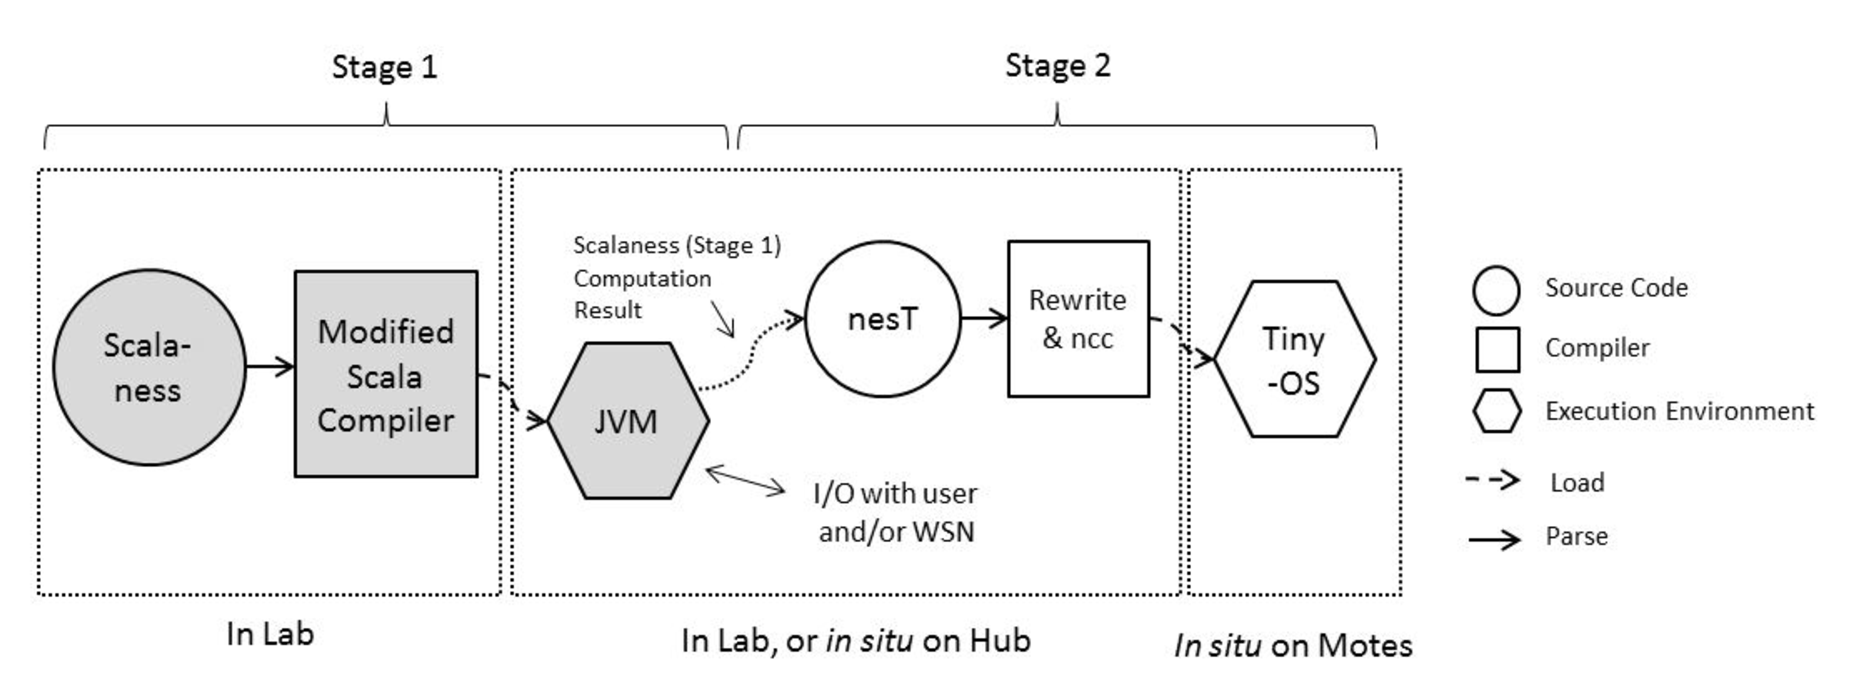
\includegraphics{scalaness}}
\begin{citemize}
\item \cemph{In the lab}: Create first stage program to specialize and compose modules of second
  stage code.
\item \cemph{In the field}: Execute first stage program to generate second stage program
  accounting for field conditions. Deploy to nodes (over the air).
\end{citemize}
\stopslide

%%%%%

\startslide{Our Approach}
\begin{citemize}
\item \cemph{Lightweight macroprogramming}. Scala at metalevel, nesC residuum.
\item Technical features: \cemph{type specialization}, \cemph{process separation}.
\item \cemph{Cross-stage type safety}: type checking at Scala level ensures type safety of nesC
  residuum.
\item \cemph{Well-founded language design}.
\end{citemize}
\stopslide

%%%%%

\startslide{Presentation Outline}
\begin{cenumerate}
\item Motivations, design overview
\item \cemph{Technical details}
\begin{citemize}
\item \cemph{Language design} 
\item Formal foundations
\end{citemize}
\item Language implementation and application
\end{cenumerate}
\stopslide

%%%%%

\startslide{Example: Introducing Some Type Abbreviations}
\lstset{basicstyle=\ttfamily, escapeinside={(*@}{@*)}}
\begin{lstlisting}[language=nesC]
(*@\tt{abbrvt\ mesgT(t) =}@*)
  { src : (*@\tt{t}@*); dest : (*@\tt{t}@*); data : uint8[] };

(*@\tt{abbrvt\ radioT =}@*)
  < at (*@$\subtype$@*) uint >
  { export error_t radio_x((*@\tt{mesgT}@*)(at)*); 
    import error_t handle_radio_r((*@\tt{mesgT}@*)(at)*); };

(*@\tt{abbrvt\ commT =}@*)
  (at (*@$\subtype$@*) uint) (*@$\circ$@*) < >
  { export error_t send((*@\tt{mesgT}@*)(at)*); 
    import error_t handle_receive((*@\tt{mesgT}@*)(at)*); };
\end{lstlisting}
\stopslide

%%%%%

\startslide{Example: nesT Modules}
\lstset{basicstyle=\ttfamily, escapeinside={(*@}{@*)}}
\begin{lstlisting}[language=nesC]
(*@\tt{authSend =}@*)
  < at (*@$\subtype$@*) uint; sendk : uint8[] >  
  { import error_t radio_x((*@\tt{mesgT}@*)(at)*);
    export error_t send(m : (*@\tt{mesgT}@*)(at)*) 
        { radio_x(AES_sign(m, sendk)); }
  };

(*@\tt{authRecv =}@*)
  < at (*@$\subtype$@*) uint; recvk : uint8[] >  
  { import error_t handle_recv((*@\tt{mesgT}@*)(at)*);
    export error_t handle_radio_r(m : (*@\tt{mesgT}@*)(at)*) 
        { if (AES_signed(m, recvk))
              handle_recv(m); }
  };
\end{lstlisting}
\stopslide

%%%%%

\startslide{Example: Scalaness Method}
\lstset{basicstyle=\ttfamily, escapeinside={(*@}{@*)}}
\begin{lstlisting}[language=scalaness]
def authSpecialize
 (nmax   : uint16,
  radioM : radioT,
  keys   : Array[Array[uint8]]) : commT {

    typedef adt (*@$\subtype$@*) uint =
      if (nmax <= 256) uint8 else uint16;

    val sendM = (*@\jinst{authSend}{adt; keys(0)}@*);
    val recvM = (*@\jinst{authRecv}{adt; keys(1)}@*);
    sendM (*@$\ltimes$@*) (*@\jinst{radioM}{adt}@*) (*@$\ltimes$@*) recvM;
}
\end{lstlisting}
\stopslide

%%%%%

\startslide{Example: Generating Residual Program}
\lstset{basicstyle=\ttfamily, escapeinside={(*@}{@*)}}
\begin{lstlisting}[language=scalaness]
val appMR =
  < >
  { export handle_recv(m : (*@\tt{mesgT}@*)(uint8)*) {(*@\ldots@*)} }; 

val appM = 
  < >
  { import send((*@\tt{mesgT}@*)(uint8)*); export main() {(*@\ldots@*)} };  

 image(appM (*@$\ltimes$@*)
         authSpecialize(nmax, radioM, keys) (*@$\ltimes$@*)
           appMR);
\end{lstlisting}
\stopslide

%%%%%

\startslide{Presentation Outline}
\begin{cenumerate}
\item Motivations, design overview
\item \cemph{Technical details}
\begin{citemize}
\item Language design 
\item \cemph{Formal foundations}
\end{citemize}
\item Language implementation and application
\end{cenumerate}
\stopslide

%%%%%

\startslide{\fml\ Foundations} The \fml\ language\footnote{\cref{Yu David Liu, Christian Skalka,
    and Scott Smith. Type-Specialized Staged Programming with Process Separation. Journal of
    Higher Order and Symbolic Computation, 24(4):341-385, 2012.}} was developed to study these
elements at a foundational level.
\begin{citemize}
\item Comprises $F_{\le}$.
\item MetaML-like syntax and semantics, but novel features to moderate interactions between
  separate process spaces.
\item Resricted form of type construction (not full $\lambda_\omega$).
\item Formal metatheory includes cross-stage type safety---residue of partial evaluation of
  well-typed code is guaranteed to be well-typed.
\end{citemize}
\stopslide

%%%%%

\startslide{Sample Scalaness Typing}
$$
\jmodt{\Delta_1}{\margs{\Delta_2, \Gamma}\lc 
  \imports; \exportsty \rc}
$$
Module type form, where:
\begin{citemize}
\item $\Delta_2$, $\Gamma$ type parameter bounds and term parameter types
\item $\imports$, $\exportsty$ import and export type signatures
\item $\Delta_1$ bounds of types constructed externally to the module
\begin{citemize}
\item Early substitution of these types unsound due to possible contravariant use in $\imports;
  \exportsty$.
\end{citemize}
\end{citemize}
$$
\inferrule[ModInstT]
{\Gamma \vdash \tt{e} : \jmodt{\varnothing}{\margs{\vect{t} \subtype \vect{\t}_1; 
 \vect{x} : \vect{\t}_2} \lc \imports; \exportsty \rc} \\
 \Gamma \vdash \ttvec{s} : \jinst{MetaType}{\ttvec{T}_1} \\
 \Gamma \vdash \ttvec{e}_2 : \ttvec{T}_2 \\
 \vdash \codt{\ttvec{T}_1} \subtype \vect{\t}_1 \\
 \vdash \codt{\ttvec{T}_2} \subtype \vect{\t}_2
}
{\Gamma \vdash \jinst{e}{\ttvec{s}; \ttvec{e}_2} : \jmodt{\ttvec{s} \subtype
    \codt{\ttvec{T}_1}}{\margs{} \lc \imports[\ttvec{s}/\vect{t}]; \exportsty[\ttvec{s}/\vect{t}] \rc} }
$$
\stopslide

%%%%%

\startslide{Presentation Outline}
\begin{cenumerate}
\item Motivations, design overview
\item Technical details
\begin{citemize}
\item Language design 
\item Formal foundations
\end{citemize}
\item \cemph{Language implementation and application}
\end{cenumerate}
\stopslide

%%%%%

\startslide{Implementation}
Scalaness/nesT has been implemented.
\begin{citemize}
\item nesT defined as restricted subset of nesC, compiled as nesC with some rewriting
  (e.g.~array bounds checks).
\item Scalaness defined by extension to the Scala compiler.
\item Type checking extends Scala type checker with module types, module operation typings, nesT
  type checking.
\end{citemize}
Web site with samples: \url{http://tinyurl.com/a85z8cu}
\stopslide

%%%%%

\startslide{Application: WSN Session Key Negotiation}
Currently studying authorization schemes for WSNs.
\begin{citemize}
\item WSN may comprise interacting security domains with different credentials and policies.
\item Symmetric keys provide efficient foundation for securing access.
\item Public keys allow symmetric key negotiation (Diffie-Hellman) in ``open world'' model.
\end{citemize}
Public key signature verification wildly expensive in WSNs; around 90 seconds on Crossbow
TelosB.

\cemph{Refactor session key negotiation and authorized access into 
different stages.}
\stopslide

%%%%%

\startslide{Application: WSN Session Key Negotiation}
\hspace*{.6in}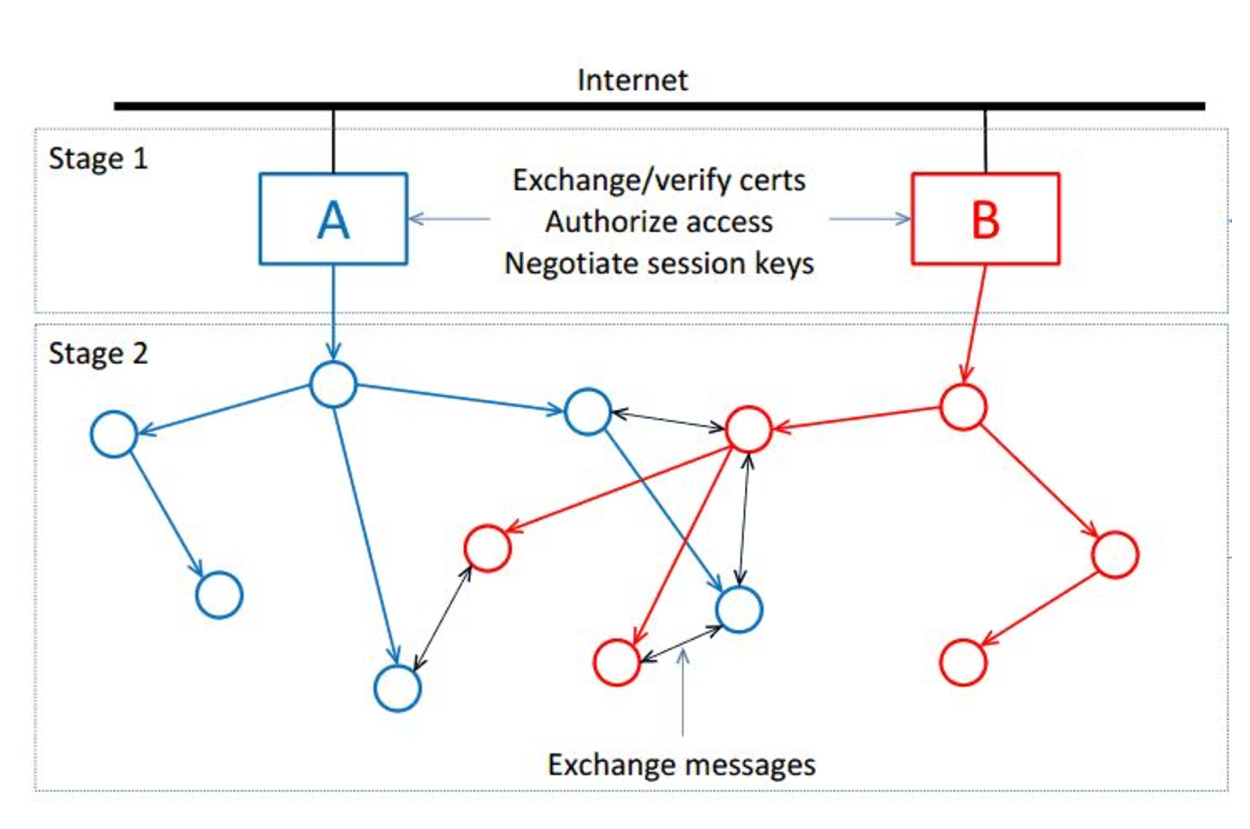
\includegraphics{spartanrpc}

Decreases WSN computational overhead, RAM and ROM consumption. 
\stopslide

%%%%%

\startslide{Results}
\begin{center}
\begin{tabular}{|r||c|c|c|c|} \hline
              & Unsecured & Unstaged* & Staged & Savings\\ \hline
Sensor ROM    &     36254 &    48616 &  36596 & 25\% \\
Sensor RAM    &      2868 &     5417 &   3038 & 44\% \\ \hline
Harvester ROM &     24316 &    35834 &  24436 & 32\% \\
Harvester RAM &      2274 &     4771 &   2402 & 50\% \\ \hline
\end{tabular}
\end{center}
\vspace{1.5in}
{\small * Chapin, Skalka; \textit{SpartanRPC}; Technical Report;
  \url{http://www.cs.uvm.edu/~skalka/skalka-pubs/chapin-skalka-spartanrpctr.pdf}}
\stopslide

%%%%%

\startslide{Future Work}
\begin{citemize}
\item Clarifying ``middle ground'' between language borders.
\item Syntactic transformations; allowing DScalaness syntax in Scalaness programs.
\item Incorporating network communication. 
\item Other applications: backcasting and evolving control.
\end{citemize}
\stopslide

%%%%%

\startslide{Questions?}
\makeatletter
\center{Peter Chapin \textless pchapin@cs.uvm.edu\textgreater}
\center{\cemph{http://tinyurl.com/a85z8cu}}
\makeatother
\stopslide
